\documentclass[11pt,aspectratio=169,xcolor=table]{beamer}

\usepackage{amsmath,amssymb}
\usepackage{graphicx}
\usepackage{xcolor}

\definecolor{ThesisBlue}{HTML}{24476F}
\definecolor{ThesisTeal}{HTML}{2F7F79}
\definecolor{ThesisGreen}{HTML}{3D7A4F}
\definecolor{ThesisRed}{HTML}{A94A4A}
\definecolor{ThesisGray}{HTML}{5F6670}
\definecolor{PaleBlue}{HTML}{EEF4F8}
\definecolor{PaleGreen}{HTML}{EDF7F0}
\definecolor{PaleRed}{HTML}{F8EEEE}
\definecolor{LineGray}{HTML}{D7DCE2}
\definecolor{FooterGray}{HTML}{8B929A}

\usefonttheme{serif}
\setbeamersize{text margin left=0.72cm,text margin right=0.72cm}
\setbeamertemplate{navigation symbols}{}
\setbeamertemplate{headline}{}
\setbeamercolor{normal text}{fg=black,bg=white}
\setbeamercolor{frametitle}{fg=ThesisBlue,bg=white}
\setbeamerfont{frametitle}{series=\bfseries,size=\large}
\setbeamercolor{eqbox}{fg=black,bg=PaleBlue}
\setbeamercolor{takeaway}{fg=black,bg=PaleGreen}
\setbeamercolor{notebox}{fg=black,bg=PaleGreen}
\setbeamercolor{footline}{fg=FooterGray,bg=white}
\setbeamercolor{itemize item}{fg=ThesisTeal}
\setbeamercolor{itemize subitem}{fg=ThesisTeal}
\setbeamercolor{enumerate item}{fg=ThesisTeal}

\setbeamertemplate{itemize item}{\raisebox{0.2ex}{\scriptsize$\blacktriangleright$}}
\setbeamertemplate{itemize subitem}{\raisebox{0.2ex}{\tiny$\blacktriangleright$}}
\setbeamertemplate{frametitle}{%
  \nointerlineskip
  \begin{beamercolorbox}[wd=\paperwidth,leftskip=0.72cm,rightskip=0.72cm,sep=0pt]{frametitle}
    \vspace{0.23cm}
    \raisebox{-4pt}[0pt][0pt]{\strut\insertframetitle\strut}\par
    \vspace{0.13cm}
    {\color{LineGray}\rule{\dimexpr\paperwidth-1.44cm\relax}{0.8pt}}
    \vspace{0.15cm}
  \end{beamercolorbox}
}
\setbeamertemplate{footline}{%
  \leavevmode
  \begin{beamercolorbox}[wd=\paperwidth,ht=2.5ex,dp=1.1ex,rightskip=0.35cm]{footline}
    \hfill\usebeamerfont{page number in head/foot}\insertframenumber
  \end{beamercolorbox}
}

\newcommand{\tealaccent}[1]{\textcolor{ThesisTeal}{\bfseries #1}}
\newcommand{\colhead}[1]{\textcolor{ThesisBlue}{\bfseries #1}}
\newcommand{\colheadgreen}[1]{\textcolor{ThesisGreen}{\bfseries #1}}
\newcommand{\smallgray}[1]{{\scriptsize\color{ThesisGray}#1}}
\newcommand{\RR}{\mathrm{RR}}
\newcommand{\MC}{\mathrm{M}}
\newcommand{\Abar}{\overline{A}}
\newcommand{\bbar}{\overline{b}}
\newcommand{\eps}{\varepsilon}

\AtBeginDocument{%
  \setlength{\abovedisplayskip}{3pt}%
  \setlength{\belowdisplayskip}{3pt}%
  \setlength{\abovedisplayshortskip}{2pt}%
  \setlength{\belowdisplayshortskip}{2pt}%
  \setlength{\jot}{2pt}%
}

\newenvironment{eqbox}
  {\begin{beamercolorbox}[wd=\linewidth,sep=0.48em,center,rounded=true]{eqbox}%
   \begin{minipage}{0.97\linewidth}\centering}
  {\end{minipage}\end{beamercolorbox}}

\newenvironment{takeawaybox}
  {\begin{beamercolorbox}[wd=\linewidth,sep=0.52em,leftskip=0.25em,rightskip=0.25em,rounded=true]{takeaway}%
   \begin{minipage}{0.96\linewidth}%
   \llap{{\color{ThesisGreen}\rule{2.5pt}{2.6ex}}\hspace{0.5em}}}
  {\end{minipage}\end{beamercolorbox}}

\newenvironment{notebox}
  {\begin{beamercolorbox}[wd=\linewidth,sep=0.42em,center,rounded=true]{notebox}%
   \begin{minipage}{0.96\linewidth}\centering}
  {\end{minipage}\end{beamercolorbox}}

\graphicspath{{figures/}}

\title{Statistical Inference for Linear Stochastic Approximation with
Richardson--Romberg Extrapolation}
\author{Danil Gainanov}
\date{2026}

\begin{document}

% ============================================================
% 1. Title
% ============================================================
\begin{frame}[plain]
  \vfill
  \begin{center}
    {\fontsize{22}{27}\selectfont\bfseries\color{ThesisBlue}
      Statistical Inference for Linear\\
      Stochastic Approximation with\\
      Richardson--Romberg Extrapolation\par}
    \vspace{1.3em}
    {\large Danil Gainanov\par}
    \vspace{0.5em}
    {\small\color{ThesisGray}Supervisor: Ilya Levin\par}
    \vspace{0.4em}
    {\small\color{ThesisGray}Master's thesis defense, 2026\par}
  \end{center}
  \vfill
\end{frame}

% ============================================================
% 2. Motivation and plan
% ============================================================
\begin{frame}[shrink=30]{Motivation: What the Recursion Solves}
\small
Linear stochastic approximation (LSA) drives \tealaccent{TD-learning and policy
evaluation} in reinforcement learning. From a \tealaccent{dependent data stream}
$Z_1,Z_2,\ldots$ (a Markov chain), the constant-step recursion
\[
  \theta_k^{(\alpha)}
  =\theta_{k-1}^{(\alpha)}
   -\alpha\bigl(A(Z_k)\theta_{k-1}^{(\alpha)}-b(Z_k)\bigr)
\]
solves the mean linear system

\begin{eqbox}
\[
  \Abar\theta^*=\bbar,\qquad
  \Abar=\mathbb{E}_{\pi}[A(Z)],\qquad
  \bbar=\mathbb{E}_{\pi}[b(Z)],\qquad
  \theta^*=\Abar^{-1}\bbar.
\]
\end{eqbox}

\vspace{0.35em}
\begin{columns}[T,onlytextwidth]
  \begin{column}{0.505\textwidth}
    \colhead{Canonical instance: TD(0).}\\[-0.2em]
    Features $\phi(s)$, $V(s)\approx\phi(s)^\top\theta$, transition
    $Z_k=(s_k,r_k,s_{k+1})$:
    \[
      A(Z_k)=\phi(s_k)\bigl(\phi(s_k)-\gamma\phi(s_{k+1})\bigr)^\top,
      \qquad b(Z_k)=r_k\phi(s_k);
    \]
    $\theta^*$ is the TD fixed point.
  \end{column}
  \begin{column}{0.465\textwidth}
    \colhead{Why inference is hard.}
    \begin{itemize}
      \item Constant step does not converge to $\theta^*$: a steady-state
      \tealaccent{bias of order $\alpha$}.
      \item A biased center invalidates a CI; no variance estimate repairs a
      wrong center.
    \end{itemize}
  \end{column}
\end{columns}

\vspace{0.2em}
\begin{takeawaybox}
Goal: a valid \textbf{confidence interval} for $u^\top\theta^*$---RR corrects
the center, long-run variance sets the width.
\end{takeawaybox}
\vspace{0.15em}
\smallgray{\textbf{Plan:} (1) setup \& target; (2) Richardson--Romberg \& the
main Berry--Esseen bound; (3) proof architecture; (4) confidence intervals
\& experiments.}
\end{frame}

% ============================================================
% 3. Setup and assumptions
% ============================================================
\begin{frame}{Setup and Assumptions}
\small
Centering the recursion at $\theta^*$ gives the \tealaccent{error recursion}

\begin{eqbox}
\[
  \theta_k^{(\alpha)}-\theta^*
  =\bigl(I-\alpha A(Z_k)\bigr)
    \bigl(\theta_{k-1}^{(\alpha)}-\theta^*\bigr)
   -\alpha\eps(Z_k),
  \qquad
  \eps(z)=\widetilde A(z)\theta^*-\widetilde b(z).
\]
\end{eqbox}

with $\widetilde A=A-\Abar$, $\widetilde b=b-\bbar$, so the noise is centered:
$\pi(\eps)=0$.

\vspace{0.45em}
\begin{columns}[T,onlytextwidth]
  \begin{column}{0.52\textwidth}
    \colhead{Assumptions}
    \begin{itemize}
      \item \textbf{(A1)} Uniform geometric ergodicity, mixing time
      $t_{\mathrm{mix}}$.
      \item \textbf{(A2)} $-\Abar$ Hurwitz; $A$, $\widetilde A$ bounded.
      \item \textbf{(A3)} Bounded noise
      $\lVert\eps\rVert_\infty<\infty$.
    \end{itemize}
  \end{column}
  \begin{column}{0.45\textwidth}
    \colhead{Polyak--Ruppert average}\\[0.15em]
    Burn-in $n_0$, window $m=n-n_0$:
    \[
      \overline\theta_{n,n_0}^{(\alpha)}
      =\frac1m\sum_{k=n_0}^{n-1}\theta_k^{(\alpha)}.
    \]
  \end{column}
\end{columns}

\vspace{0.35em}
\smallgray{Markovian noise means the randomness in $A(Z_k)$, $b(Z_k)$ is
serially dependent; the constant step $\alpha$ does not vanish, so the
iterates have a steady-state bias.}
\end{frame}

% ============================================================
% 4. Statistical target and error sources
% ============================================================
\begin{frame}{Statistical Target and Two Error Sources}
\small
For confidence intervals we need a normal approximation for scalar projections
\[
  \sqrt n\,u^\top(\overline\theta_n-\theta^*)
  \approx\mathcal N(0,u^\top\Sigma_\infty u).
\]
Two distinct obstacles:

\vspace{0.5em}
\begin{columns}[T,onlytextwidth]
  \begin{column}{0.48\textwidth}
    \colhead{Centering error}
    \[
      \mathbb E\,\overline\theta_n^{(\alpha)}-\theta^*
      =\alpha\Delta+\text{higher order}.
    \]
    A variance estimator cannot correct a biased interval center.
  \end{column}
  \begin{column}{0.48\textwidth}
    \colhead{Dependent fluctuation}
    \[
      \Sigma_\eps^{\MC}
      =\mathbb E[\eps_0\eps_0^\top]
       +2\sum_{\ell\geq1}\mathbb E[\eps_0\eps_\ell^\top].
    \]
    The normal variance must include serial correlations.
  \end{column}
\end{columns}

\vspace{0.65em}
\begin{takeawaybox}
Two separate tasks: \textbf{correct the center} of the estimator, and
\textbf{approximate the dependent-noise distribution} around that center.
RR handles the first.
\end{takeawaybox}
\end{frame}

% ============================================================
% 5. Richardson--Romberg
% ============================================================
\begin{frame}{Richardson--Romberg in the Step Size}
\small
Run two PR-averaged LSA trajectories on the \tealaccent{same Markov chain path},
with steps $\alpha$ and $2\alpha$, and extrapolate:
\[
  \overline\theta_n^\RR
  =2\overline\theta_n^{(\alpha)}-\overline\theta_n^{(2\alpha)}.
\]

Both branches carry the same leading bias slope $\Delta$ (Levin et al., 2025),
so the linear term cancels:

\begin{eqbox}
\[
  \overline\theta_n^{(\alpha)}\approx\theta^*+\alpha\Delta,\qquad
  \overline\theta_n^{(2\alpha)}\approx\theta^*+2\alpha\Delta
  \quad\Longrightarrow\quad
  \overline\theta_n^\RR
  \approx\theta^*+(2\alpha-2\alpha)\Delta
  =\theta^*+O(\alpha^{3/2}).
\]
\end{eqbox}

\vspace{0.55em}
\begin{takeawaybox}
RR moves the \textbf{center} of the confidence interval; it does not estimate
the covariance. The shared path keeps the two branches' noise highly
correlated, so extrapolation cancels bias instead of adding simulation error.
\end{takeawaybox}
\end{frame}

% ============================================================
% 6. Inference target
% ============================================================
\begin{frame}[shrink=6]{What Distribution Should We Approximate?}
\small
For a direction $u$ and window $m=n-n_0$, the practical statistic is

\begin{eqbox}
\[
  \sqrt m\,u^\top(\overline\theta_{n,n_0}^\RR-\theta^*)
  \quad\Longrightarrow\quad
  \mathcal N(0,\sigma^2(u)),
  \qquad \sigma^2(u)=u^\top\Sigma_\infty u.
\]
\end{eqbox}

\vspace{0.55em}
Because the data are dependent, the target is the \tealaccent{long-run}
covariance, not a one-step variance:
\[
  \Sigma_\infty
  =\Abar^{-1}\Sigma_\eps^\MC\Abar^{-\top},
\]
\[
  \Sigma_\eps^\MC
  =\mathbb E_\pi[\eps_0\eps_0^\top]
   +\sum_{j\geq1}\left(
      \mathbb E_\pi[\eps_0\eps_j^\top]
      +\mathbb E_\pi[\eps_j\eps_0^\top]\right).
\]

\vspace{0.45em}
\begin{takeawaybox}
The inference goal is a Gaussian approximation of the scalar RR statistic
with the Markovian long-run variance
$\sigma^2(u)=u^\top\Sigma_\infty u$.
\end{takeawaybox}
\end{frame}

% ============================================================
% 7. Main result
% ============================================================
\begin{frame}[shrink=2]{Main Theoretical Result}
\small
Under (A1)--(A3), at the \tealaccent{balanced scale}
$\alpha=cn^{-1/2}$ with burn-in
$n_0\asymp(\alpha a)^{-1}\log^2n$---where $c>0$ is the step-size constant
and $a$ the Lyapunov contraction rate---the burned-in RR average satisfies a
Berry--Esseen bound:

\begin{eqbox}
\[
  d_{\mathrm K}\!\left(
    \frac{\sqrt m\,u^\top
      (\overline\theta_{n,n_0}^\RR-\theta^*)}{\sigma(u)},
    \mathcal N(0,1)\right)
  \leq C(u,c,\theta_0)\,
       \operatorname{polylog}(n)\,n^{-1/4},
  \qquad
  \sigma^2(u)=u^\top\Sigma_\infty u.
\]
\end{eqbox}

\vspace{0.55em}
\begin{takeawaybox}
The theorem turns the RR averaged estimator into a valid
normal-approximation object for scalar confidence intervals.
\end{takeawaybox}

\vspace{0.3em}
\smallgray{The constant $C(u,c,\theta_0)$ depends only on the direction $u$,
the step-size constant $c$ in $\alpha=cn^{-1/2}$, and the start $\theta_0$.
The $n^{-1/4}$ rate is the martingale Berry--Esseen rate; polylog factors
absorb the mixing time and the burn-in.}
\end{frame}

% ============================================================
% 8a. Theorem I (1/3): decomposition and weights
% ============================================================
\begin{frame}[shrink=10]{Theorem I (1/3): Decomposition and RR Weights}
\footnotesize
In the stationary augmented chain ($n_0=0$), unfolding the error recursion and
PR-averaging splits the scaled error into a noise sum plus deterministic
remainders:

\begin{eqbox}
\[
  \sqrt n\,(\overline\theta_n^\RR-\theta^*)=W^\RR+D^\RR,
  \qquad
  W^\RR=-\frac1{\sqrt n}\sum_{\ell=1}^{n-1}
    \mathcal Q_\ell^\RR\,\eps(Z_\ell).
\]
\end{eqbox}

The deterministic \textbf{RR weight} is
$\mathcal Q_\ell^\RR=2Q_\ell^{(\alpha)}-Q_\ell^{(2\alpha)}$, with
$Q_\ell^{(\alpha)}=\Abar^{-1}(I-B_\alpha^{n-\ell})$ and
$B_\alpha=I-\alpha\Abar$ (write $k=n-\ell$):

\vspace{0.25em}
\begin{columns}[T,onlytextwidth]
  \begin{column}{0.49\textwidth}
    \colhead{Closeness to $\Abar^{-1}$}
    \[
      \mathcal Q_\ell^\RR-\Abar^{-1}
      =-\Abar^{-1}(2B_\alpha^k-B_{2\alpha}^k),
    \]
    \[
      \sum_\ell\lVert\mathcal Q_\ell^\RR-\Abar^{-1}\rVert^2
      \leq\frac{C_1}{\alpha a}.
    \]
  \end{column}
  \begin{column}{0.47\textwidth}
    \colhead{Bounded variation}
    \[
      \sum_\ell\lVert
        \mathcal Q_{\ell+1}^\RR-\mathcal Q_\ell^\RR
      \rVert\leq\frac{C_2}{a^2}.
    \]
    Controls the Abel / Poisson boundary remainder.
  \end{column}
\end{columns}

\vspace{0.2em}
\begin{takeawaybox}
All stochastic content of the leading term sits in $\eps(Z_\ell)$; the kernel
is deterministic and asymptotically $\Abar^{-1}$.
\end{takeawaybox}
\end{frame}

% ============================================================
% 8b. Theorem I (2/3): Poisson martingale and variance
% ============================================================
\begin{frame}[shrink=10]{Theorem I (2/3): Poisson Martingale and Variance}
\footnotesize
$W^\RR$ is a dependent sum. Solve the \textbf{Poisson equation}
$\widehat\eps-\mathsf Q\widehat\eps=\eps$ and split each $\eps(Z_\ell)$ into
a martingale increment plus a telescoping term; Abel summation gives

\begin{eqbox}
\[
  W^\RR=-\frac1{\sqrt n}M_n^\RR+D_{2,n}^\RR,\qquad
  \Delta M_\ell^\RR
  =\mathcal Q_\ell^\RR
    \bigl(\widehat\eps(Z_\ell)-\mathsf Q\widehat\eps(Z_{\ell-1})\bigr),
\]
\end{eqbox}

where the Abel remainder is
$\lVert D_{2,n}^\RR\rVert_{L^p}=O(t_{\mathrm{mix}}n^{-1/2})$.

\vspace{0.25em}
\begin{columns}[T,onlytextwidth]
  \begin{column}{0.49\textwidth}
    \colhead{Variance matches the target}
    \[
      \Sigma_n^\RR=\frac1n\sum_{\ell=2}^{n-1}
      \mathcal Q_\ell^\RR\Sigma_\eps^\MC
      (\mathcal Q_\ell^\RR)^\top,
    \]
    \[
      \lVert\Sigma_n^\RR-\Sigma_\infty\rVert
      \leq\frac{C_3}{n\alpha a}.
    \]
  \end{column}
  \begin{column}{0.47\textwidth}
    \colhead{Martingale Berry--Esseen}
    \[
      d_{\mathrm K}\!\left(
        \frac{u^\top M_n^\RR}
             {\sqrt n\,\sigma_n^\RR(u)},\mathcal N(0,1)\right)
      \leq\frac{C\log^{3/4}n}{n^{1/4}}
          +\frac{C\log n}{\sqrt n}.
    \]
  \end{column}
\end{columns}

\vspace{0.15em}
\begin{takeawaybox}
The dependent fluctuation reduces to a bounded-increment martingale whose
variance is $\Sigma_\infty$ up to $O(1/(n\alpha a))$.
\end{takeawaybox}
\end{frame}

% ============================================================
% 8c. Theorem I (3/3): misadjustment and assembly
% ============================================================
\begin{frame}[shrink=25]{Theorem I (3/3): Misadjustment and Assembly}
\footnotesize
The remaining non-martingale piece is the RR \textbf{misadjustment}
\[
  R_n^{\mathrm{mis,RR}}
  =\frac1{\sqrt n}\sum_{k=0}^{n-1}
    \bigl(2R_k^{(\alpha)}-R_k^{(2\alpha)}\bigr).
\]
A depth-two refinement of the perturbation recursions (Levin et al., 2025)
controls it at the same order as the martingale rate:

\begin{eqbox}
\[
  \lVert R_n^{\mathrm{mis,RR}}\rVert_{L^p}
  \leq C\,\operatorname{polylog}(n)\,n^{-1/4}
  \qquad\text{at}\qquad \alpha=cn^{-1/2}.
\]
\end{eqbox}

\vspace{0.4em}
A Bobkov--Götze \textbf{smoothing inequality} then merges the martingale
Berry--Esseen term and this remainder into a single Kolmogorov bound,
\[
  d_{\mathrm K}(X_n+Y_n,\mathord{\cdot})
  \leq d_{\mathrm K}(X_n,\mathord{\cdot})
      +\frac{e\lVert Y_n\rVert_{L^p}}{\sqrt{2\pi}}+e^{-p}.
\]

\vspace{0.35em}
\begin{takeawaybox}
Stationary balanced-scale bound:
\[
  d_{\mathrm K}\!\left(
    \frac{S_{n,\mathrm{stat}}^\RR(u)}{\sigma_n^\RR(u)},
    \mathcal N(0,1)\right)
  \leq C(u)\operatorname{polylog}(n)n^{-1/4},
\]
with covariance target $\Sigma_\infty$.
\end{takeawaybox}
\end{frame}

% ============================================================
% 9. Burn-in theorem
% ============================================================
\begin{frame}{Theorem II: Burn-in Transfer to Deterministic Starts}
\footnotesize
The real algorithm starts from a fixed $\theta_0$ and a non-stationary $Z_0$.
We transfer the stationary bound to the burned-in statistic
\[
  T_{n,n_0}^\RR(u)
  =\sqrt m\,u^\top(\overline\theta_{n,n_0}^\RR-\theta^*),
  \qquad m=n-n_0.
\]

\vspace{0.2em}
\begin{columns}[T,onlytextwidth]
  \begin{column}{0.50\textwidth}
    \colhead{Four extra sources, all controlled}
    \begin{itemize}
      \item deterministic transient $B_\alpha^k(\theta_0-\theta^*)$;
      \item random initial products
      $\Gamma_{1:k}^{(\alpha)}-B_\alpha^k$;
      \item augmented-chain startup discrepancy;
      \item finite-window variance normalization.
    \end{itemize}
  \end{column}
  \begin{column}{0.45\textwidth}
    \colhead{Balanced burn-in result}\\[0.2em]
    With $n_0\asymp(\alpha a)^{-1}\log^2n$ and
    $\alpha=cn^{-1/2}$:
    \begin{eqbox}
    \resizebox{0.92\linewidth}{!}{$\displaystyle
      d_{\mathrm K}\!\left(
        \Xi_{n,n_0}^\RR(u),\mathcal N(0,1)\right)
      \leq C(u,c,\theta_0)\operatorname{polylog}(n)n^{-1/4}.
    $}
    \end{eqbox}
  \end{column}
\end{columns}

\vspace{0.35em}
\begin{takeawaybox}
This is the theorem behind the estimator used in experiments: discard the
burn-in, average the remaining RR iterates, and use the same covariance target
$\Sigma_\infty$.
\end{takeawaybox}
\end{frame}

% ============================================================
% 10. Practical intervals
% ============================================================
\begin{frame}{From Theory to Confidence Intervals}
\small
In practice $\Sigma_\infty$ is unknown, so the long-run variance of the
projected trajectory $Y_t=u^\top\theta_t$ is estimated from one dependent run.

\vspace{0.5em}
\begin{columns}[T,onlytextwidth]
  \begin{column}{0.485\textwidth}
    \colhead{OBM} (overlapping batch means, block $b$)
    \[
      \widehat\sigma_{\mathrm{OBM}}^2(b)
      =\frac{b}{T-b+1}\sum_{s=0}^{T-b}
        \bigl(\overline Y_{s,b}-\overline Y_T\bigr)^2.
    \]
    Window bias $\approx c_1(u)/b$, often negative.
  \end{column}
  \begin{column}{0.485\textwidth}
    \colhead{OBM-LW / lugsail} ($\lambda>1$)
    \[
      \widehat\sigma_{\mathrm{LW}}^2
      =\frac{\lambda}{\lambda-1}\widehat\sigma_{\mathrm{OBM}}^2(\lambda b)
       -\frac1{\lambda-1}\widehat\sigma_{\mathrm{OBM}}^2(b).
    \]
    $\lambda=2$ cancels the leading $1/b$ bias.
  \end{column}
\end{columns}

\vspace{0.65em}
\begin{takeawaybox}
\textbf{RR changes the center; OBM and lugsail change the width.} The thesis
proves the RR distributional approximation; non-asymptotic OBM/lugsail theory
along RR trajectories is left as future work.
\end{takeawaybox}
\end{frame}

% ============================================================
% 11. Experiments setup
% ============================================================
\begin{frame}[shrink=5]{Numerical Experiments}
\small
\renewcommand{\arraystretch}{1.18}
\begin{center}
\begin{tabular}{|p{0.30\textwidth}|p{0.61\textwidth}|}
  \hline
  \rowcolor{PaleBlue}\textbf{Quantity} & \textbf{Main setup}\\ \hline
  Problem class & Finite-state Markovian LSA\\ \hline
  Dimension and states & $d=5$, 10 Markov states\\ \hline
  Monte Carlo design & 100 problems, 100 trajectories per problem\\ \hline
  Trajectory length & $T=10^6$\\ \hline
  RR stepsizes & $\alpha\in\{0.2,0.02\}$ in the main comparison\\ \hline
  Inference & 95\% scalar intervals in a random projection direction\\ \hline
  Variance estimators & Batch means, OBM, OBM-LW, MSB, and oracle diagnostics\\ \hline
\end{tabular}
\end{center}

\vspace{0.4em}
\begin{takeawaybox}
The experiments are designed to separate the point-estimator bias from the
long-run variance estimation error.
\end{takeawaybox}
\end{frame}

% ============================================================
% 12. Main comparison
% ============================================================
\begin{frame}{Main Comparison: RR Fixes the Center}
\scriptsize
\begin{columns}[T,onlytextwidth]
  \begin{column}{0.44\textwidth}
    \renewcommand{\arraystretch}{1.16}
    \begin{tabular}{|l|c|c|}
      \hline
      \rowcolor{PaleBlue}\textbf{Method}&\textbf{L2}&\textbf{Cov.}\\ \hline
      $\alpha=0.2$ const.&$26.67$&$0.5\%$\\ \hline
      $\alpha=0.02$ const.&$13.93$&$40.5\%$\\ \hline
      \rowcolor{PaleGreen}RR const.&$4.52$&$94.0\%$\\ \hline
      Diminishing&$6.80$&$90.0\%$\\ \hline
      PR + OBM&$5.35$&$92.0\%$\\ \hline
      \rowcolor{PaleGreen}RR + OBM&$4.52$&$95.0\%$\\ \hline
      \rowcolor{PaleGreen}RR + OBM-LW&$4.52$&$95.0\%$\\ \hline
    \end{tabular}

    \vspace{0.45em}
    \smallgray{L2 is reported in units of $10^{-3}$; medians over 100
    problems.}
  \end{column}
  \begin{column}{0.54\textwidth}
    \centering
    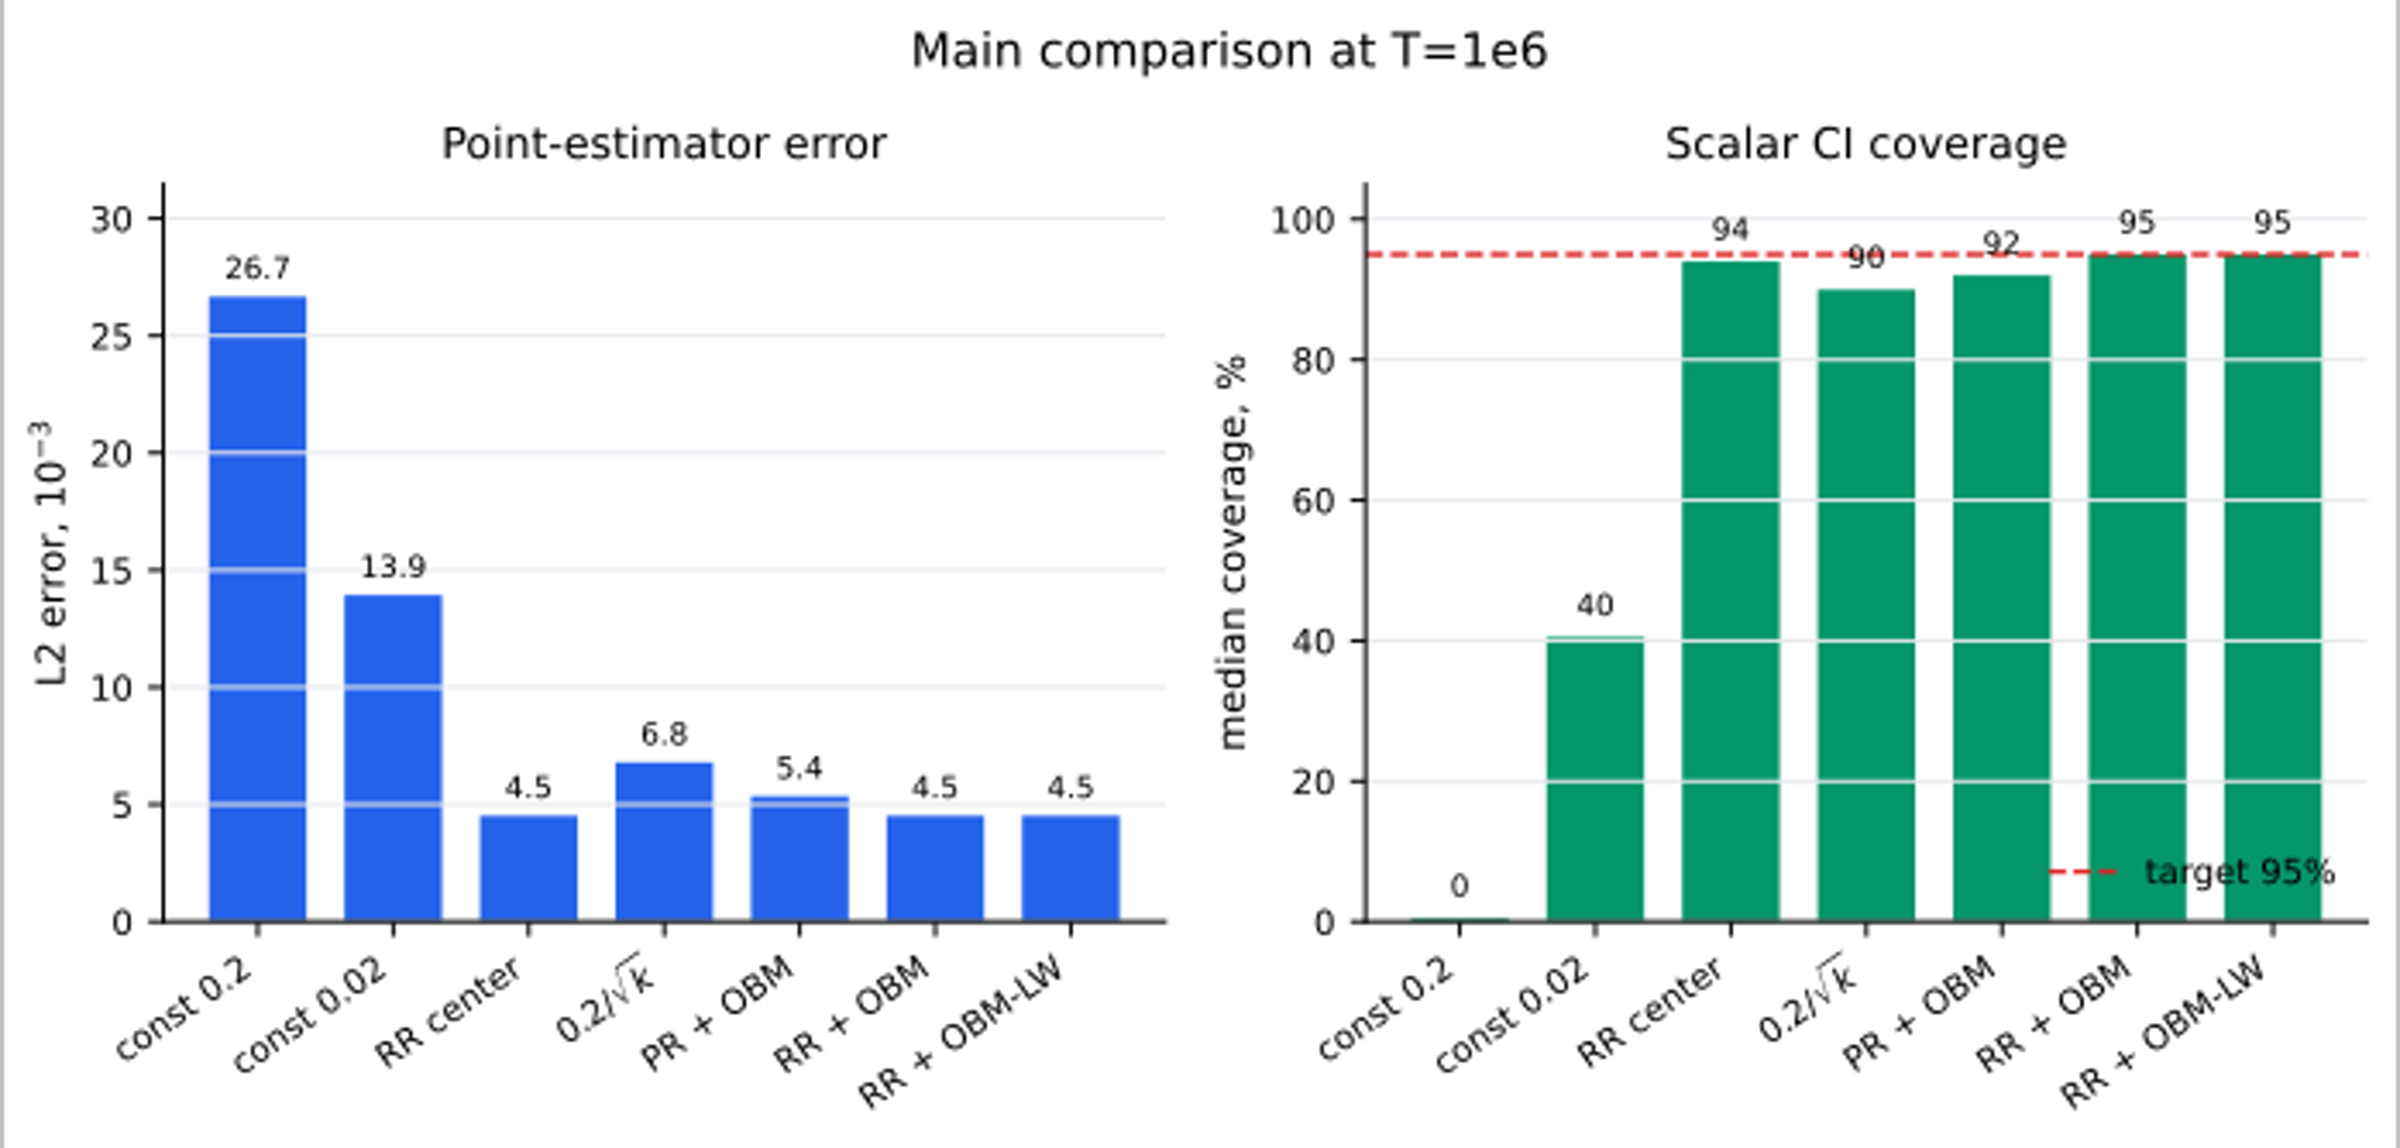
\includegraphics[width=\linewidth]{main_methods_comparison.png}
  \end{column}
\end{columns}

\vspace{0.35em}
\begin{takeawaybox}
The coverage gain is not achieved by widening intervals: RR mainly improves
the interval center by reducing step-size bias.
\end{takeawaybox}
\end{frame}

% ============================================================
% 13. Stepsize and oracle diagnostics
% ============================================================
\begin{frame}{Diagnostics: Stepsize and Variance Estimation}
\footnotesize
\renewcommand{\arraystretch}{1.18}
\begin{center}
\resizebox{0.98\linewidth}{!}{%
\begin{tabular}{|l|l|c|c|}
  \hline
  \rowcolor{PaleBlue}
  \textbf{RR pair}&\textbf{Single-step coverage}&\textbf{RR L2}&
  \textbf{RR cov.}\\ \hline
  \rowcolor{PaleGreen}
  $(0.04,0.02)$&$0.04$: $92.0\%$; $0.02$: $94.0\%$&$2.97$&$94.0\%$\\ \hline
  \rowcolor{PaleGreen}
  $(0.10,0.05)$&$0.10$: $86.0\%$; $0.05$: $91.5\%$&$2.97$&$94.0\%$\\ \hline
  \rowcolor{PaleGreen}
  $(0.20,0.10)$&$0.20$: $67.5\%$; $0.10$: $86.0\%$&$2.97$&$94.0\%$\\ \hline
\end{tabular}}
\end{center}

\vspace{0.45em}
For the largest adjacent pair, oracle and practical variance intervals are
almost identical:

\begin{notebox}
RR + oracle variance: 95.0\%; RR + OBM: 95.0\%; RR + MSB: 95.0\% coverage.
\end{notebox}

\vspace{0.35em}
\smallgray{Across $T\in\{2\cdot10^4,\ldots,10^6\}$ the oracle interval stays
near $95\%$ coverage, so the RR center and the normal approximation are not
the bottleneck. The only short-horizon gap is variance estimation: at
$T=2\cdot10^4$ the data-driven interval is about $5.8\%$ too narrow, and this
gap closes as $T$ grows.}
\end{frame}

% ============================================================
% 14. OBM and lugsail
% ============================================================
\begin{frame}{Variance Estimation: When Does Lugsail Help?}
\footnotesize
\begin{columns}[T,onlytextwidth]
  \begin{column}{0.44\textwidth}
    The remaining short-horizon gap is in \textbf{variance estimation}, not
    the center.

    \vspace{0.45em}
    \textbf{OBM can be too narrow} when the Bartlett-window bias is negative.

    \vspace{0.45em}
    \textbf{Lugsail helps at small blocks / short horizons:} at
    $T=2\cdot10^4$, $\eta=0.5$ it lifts median coverage
    $91.5\%\to95.0\%$.

    \vspace{0.45em}
    \textbf{But not automatic:} neutral at the production rule $\eta=0.6$,
    and the signed estimate can turn negative for very large blocks.
  \end{column}
  \begin{column}{0.54\textwidth}
    \centering
    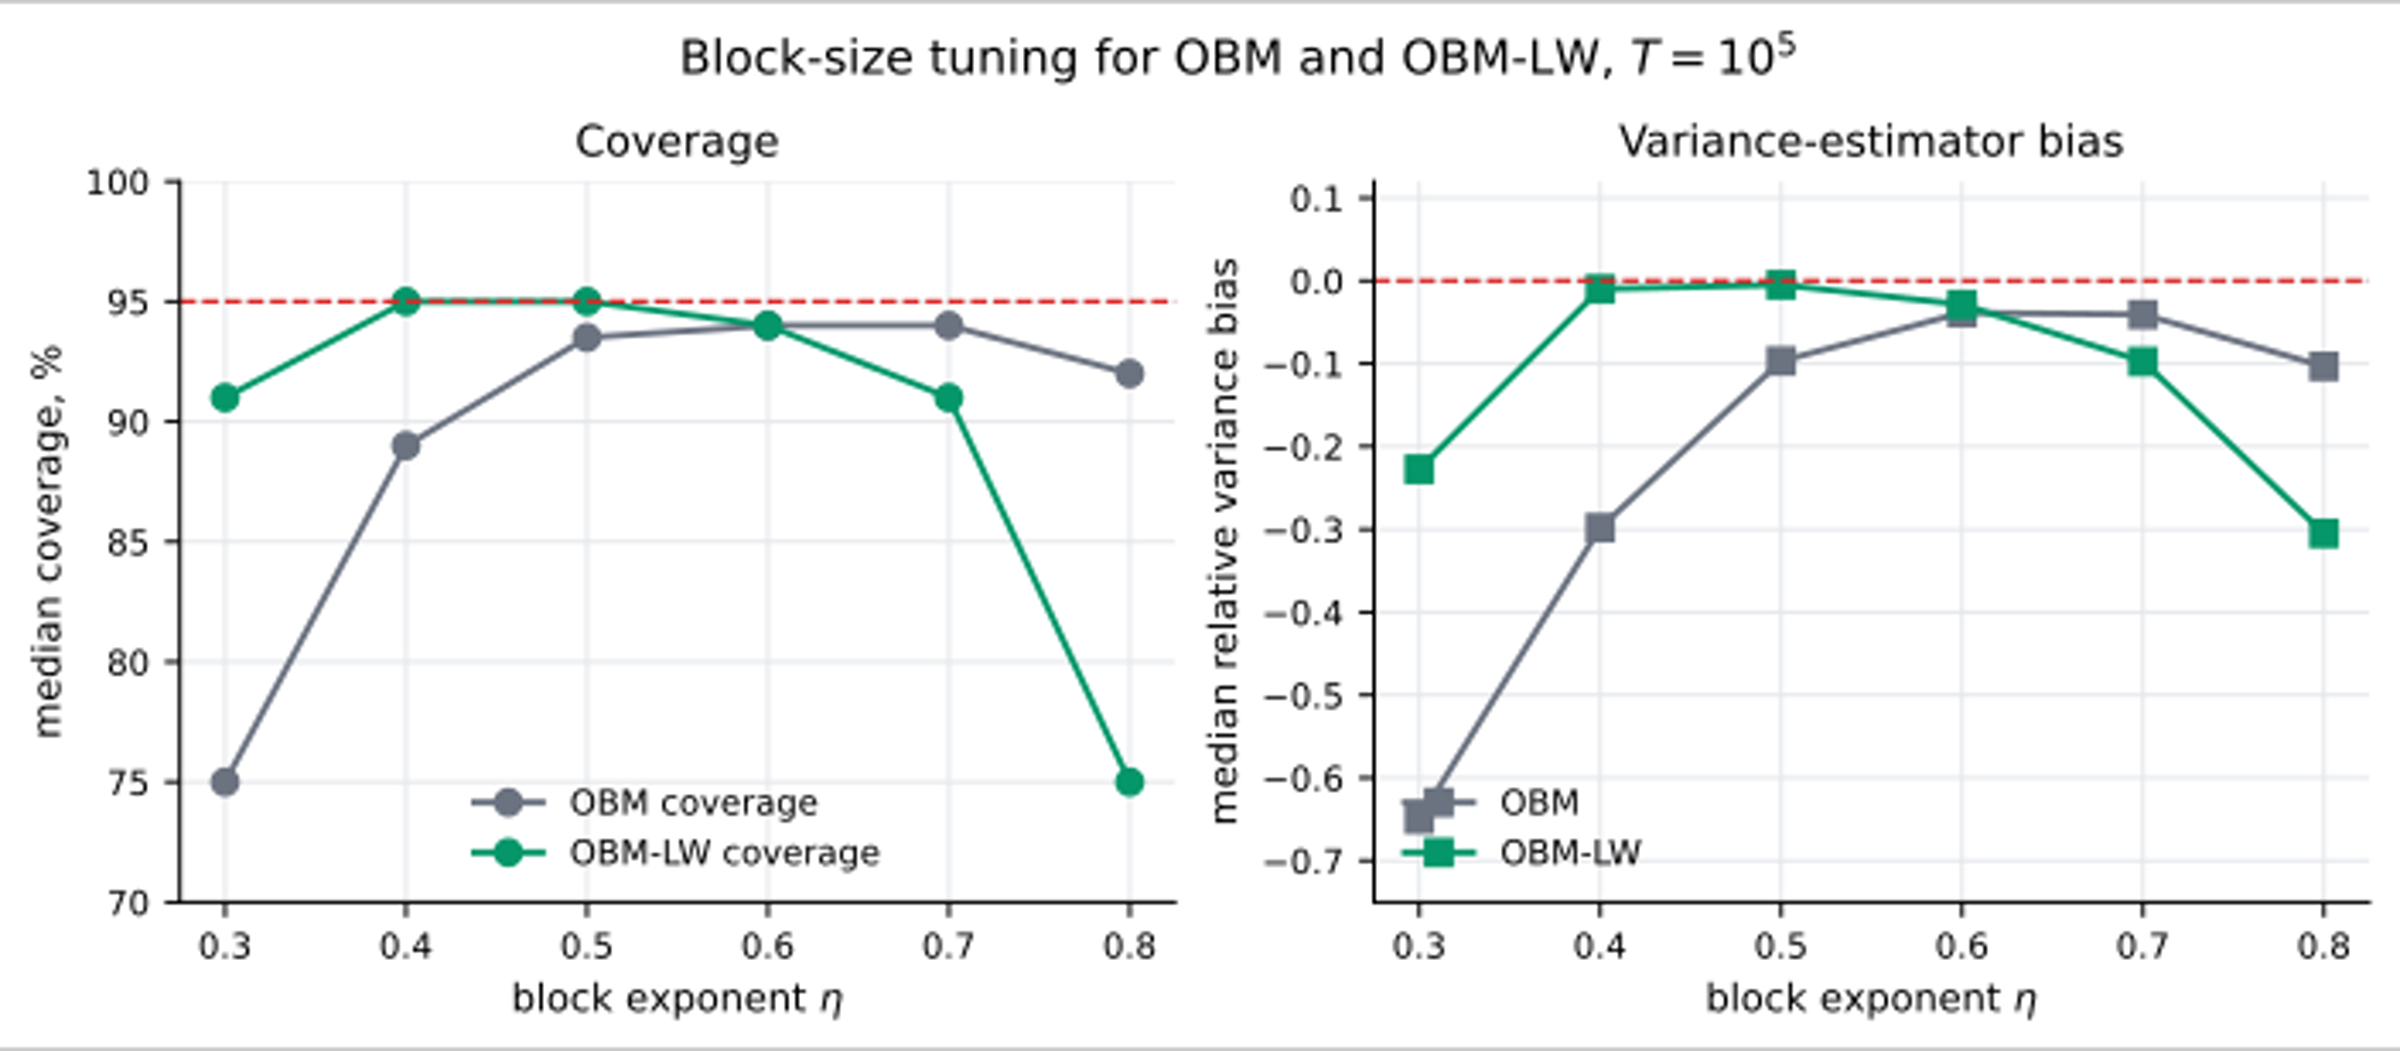
\includegraphics[width=\linewidth]{blocksize_lugsail_diagnostics.png}
  \end{column}
\end{columns}

\vspace{0.3em}
\begin{takeawaybox}
Step-size RR and lugsail OBM solve different problems: center bias versus
variance-estimator window bias.
\end{takeawaybox}
\end{frame}

% ============================================================
% 15. Contributions
% ============================================================
\begin{frame}[shrink=2]{Contributions and Limitations}
\small
\begin{columns}[T,onlytextwidth]
  \begin{column}{0.49\textwidth}
    \colhead{Main contributions}
    \begin{itemize}
      \item Formulated RR-averaged constant-step LSA inference under
      Markovian noise.
      \item Proved a scalar Berry--Esseen bound at the balanced scale.
      \item Transferred the result from stationary starts to burned-in
      deterministic starts.
      \item Verified the bias-correction mechanism in finite-state
      experiments.
    \end{itemize}
  \end{column}
  \begin{column}{0.47\textwidth}
    \colhead{Limitations and future work}
    \begin{itemize}
      \item Full multivariate confidence regions.
      \item Non-asymptotic OBM and lugsail theory along RR trajectories.
      \item Sharper dependence on mixing time and stability constants.
      \item More diagnostics for slow mixing and matrix covariance estimates.
    \end{itemize}
  \end{column}
\end{columns}

\vspace{0.5em}
\begin{takeawaybox}
The central message: RR makes constant-step LSA statistically usable by
correcting the center, while standard long-run variance tools handle the
interval width.
\end{takeawaybox}
\end{frame}

% ============================================================
% 16. Thank you
% ============================================================
\begin{frame}[plain]
  \vfill
  \begin{center}
    {\fontsize{26}{31}\selectfont\bfseries\color{ThesisBlue}Thank you!\par}
    \vspace{0.9em}
    {\Large\color{ThesisGray}Questions?\par}
  \end{center}
  \vfill
\end{frame}

\end{document}
